%% -*- coding: utf-8; -*-
\documentclass[phd,brazilian]{ThesisPUC}

%---------- Math ----------%
\usepackage{amsmath}
\usepackage{amssymb}
\usepackage{mathtools}
\usepackage{bbm}
%---------- Floating ----------%
\usepackage{float}
%---------- Algorithm ----------%
\usepackage[algosection, algoruled]{algorithm2e}
%---------- Tables ----------%
\usepackage{multicol}
\usepackage{booktabs}
%---------- TiKz ----------%
\usepackage{threeparttable}
\usepackage{standalone}
\usepackage{xcolor}
\usepackage{tikz}
\usepackage{psfrag,epsf}
\usepackage{multirow}

\graphicspath{{../../common/images/}}

%---------- Cover ----------%
\author{Guilherme Gonçalves Schardong}
\authorR{Schardong, Guilherme Gonçalves}
\advisor{Hélio Côrtes Vieira Lopes}{Prof.}
\advisorR{Lopes, Hélio Côrtes Vieira}
\coadvisor{Simone Diniz Junqueira Barbosa}{Prof$^{\text{a}}$.}
\coadvisorR{Barbosa, Simone Diniz Junqueira}

% The \usecolour command adds the "(Cor)" token in the thesis catalographic sheets and should be included if the thesis contains figures in RGB color.
\usecolour{true}
\title{Uma Abordagem Visual e Interativa para a Seleção de Conjuntos de Cenários Temporais}
\titleuk{Visual interactive support for selecting scenarios from time-series ensembles}

\day{13}
\month{Setembro}
\myyear{2018}

\city{Rio de Janeiro}
\CDD{004} % Fill this number by calling the PUC-Rio central library.
\department{Informática}
\program{Informática}
\school{Centro Técnico Científico}
\university{Pontifícia Universidade Católica do Rio de Janeiro}
\uni{PUC-Rio}

%---------- Jury ----------%
%% The \jury command declares the members of the evaluation comitee for the thesis and is mandatory.
%% The \jurymember command declares a jury member from the university itself.
%% The \extjurymember command declares a jury member from outside the university. These members cannot have their department listed.
\jury{
  \jurymember{Fernando Luiz Cyrino Oliveira}{Prof.}{Departamento de Engenharia Industrial}{PUC-Rio}
  \jurymember{Bruno Fânzeres dos Santos}{Prof.}{Departamento de Engenharia Industrial}{PUC-Rio}
  \extjurymember{Regis Kruel Romeu}{Prof.}{CENPES}
  \extjurymember{Sergio Lima Netto}{Prof.}{UFRJ}
  \jurymember{Abelardo Borges Barreto Junior}{Prof.}{Departamento de Matemática}{PUC-Rio}
  \extjurymember{Alex Laier Bordignon}{Prof.}{UFF}
  \schoolhead{Márcio da Silveira Carvalho}{Prof.}
}

%---------- Front letters ----------%
\resume
{
  Bacharel em Ciência da Computação (2011) e Mestre em Informática com ênfase em Computação aplicada (2014) pela Universidade Federal de Santa Maria (UFSM). Atuou no Laboratório de Computação Aplicada (LaCA-UFSM) de 2009 a 2014 e no Instituto Tecgraf de 2014 a 2016 durante o doutorado. De 2016 até o momento, atua no GALGOS/ATD-Lab na PUC-Rio.
}

%% The \acknowledgement command is optional. This example includes a statement for CAPES and CNPq and should be included if the student was financed by any of these organizations.
\acknowledgment
{
  \noindent
  Ao Conselho Nacional de Desenvolvimento Científico e Tecnológico (CNPq) por financiar parcialmente essa pesquisa sob o contrato XXXXXX/YYYY-X. \\
  \noindent
  O presente trabalho foi realizado com apoio da Coordenação de Aperfeiçoamento de Pessoal de Nível Superior - Brasil (CAPES) - Código de Financiamento 001. \\
}

%% The \keywords and \keywordsuk commands declare the keywords to be include in the thesis catalographic sheets, while the \keywordsabstract* commands declare the same keywords but for the thesis abstracts.
%% This is a terrible hack and should be fixed in order to avoid unnecessary repetition
\keywords
{
  \key{Redução de Cenários}
  \key{Interatividade}
  \key{Visualização Científica}
  \key{Tomada de Decisão}
  \key{Conjuntos de Dados Temporais}
}

\keywordsabstract
{
  \key{Redução de Cenários;}
  \key{Interatividade;}
  \key{Visualização Científica;}
  \key{Tomada de Decisão;}
  \key{Conjuntos de Dados Temporais.}
}

\keywordsuk
{
  \key{Scenario Reduction}
  \key{User Interaction}
  \key{Scientific Visualization}
  \key{Decision Making}
  \key{Time Series Ensembles}
}

\keywordsabstractuk
{
  \key{Scenario Reduction;}
  \key{User Interaction;}
  \key{Scientific Visualization;}
  \key{Decision Making;}
  \key{Time Series Ensembles.}
}

% The abstract and abstractuk commands declare the portuguese and english abstracts respectively. The thesis language sets which abstact will be shown first (portuguese if the thesis is in portuguese, same for english). However, the declaration can be done in any order. Both are mandatory.
\abstract{
  O uso de abordagens de programação estocástica e redução de cenários tem se tornado imprescindível na análise e predição de comportamento de sistemas dinâmicos. Entretanto, tais técnicas não levam em conta o conhecimento prévio sobre domínio que o usuário possui. O presente trabalho tem por objetivo o desenvolvimento de uma abordagem visual e interativa para abordar o problema de redução de cenários com dados temporais. Para tanto, nós propomos a implementação de uma série de visualizações de dados temporais integradas. Também propomos a adaptação de um algoritmo de projeção multidimensional para lidar com dados temporais. Desta forma, podemos representar graficamente a evolução de um conjunto de cenários ao longo do tempo. Outra visualização proposta no presente trabalho é uma adaptação de \textit{Bump chart} para lidar com dados temporais acumulados; através dele, um usuário pode comparar a evolução das distâncias entre os diferentes cenários e um cenário de referência. Para validar a nossa proposta, fizemos uma implementação das técnicas propostas e conduzimos um estudo com usuários de diferentes áreas do conhecimento e níveis de experiência. Os resultados obtidos até então indicam que uma abordagem visual para o problema de redução de cenários é viável, e permite a seleção de um conjunto razoável de cenários. Além disso, constatamos que essa abordagem pode ser útil em um contexto de exploração de dados visando a redução de cenários. O usuário também pode explorar visualmente os resultados de outras técnicas de redução de cenários usando nossa abordagem. Os usuários entrevistados reportaram facilidade em cumprir as tarefas propostas e comentaram positivamente sobre os mecanismos de interação fornecidos pelo nosso protótipo. Também testamos os cenários escolhidos usando nossa proposta contra outras abordagens encontradas tanto na literatura quanto em uso na indústria. Os resultados obtidos foram bons, indicando que nossa proposta é viável em casos de uso reais.
}

\abstractuk{
  Stochastic programming and scenario reduction approaches have become invaluable in the analysis and behavior prediction of dynamic systems. However, such techniques often fail to take advantage of the user's own expertise about the problem domain. This work provides visual interactive support to assist users in solving the scenario reduction problem with time-series data. We employ a series of time-based visualization techniques linked together to perform the task. By adapting a multidimensional projection algorithm to handle temporal data, we can graphically present the evolution of the ensemble. We also propose to use cumulative bump charts to visually compare the ranks of distances between the ensemble time series and a baseline series. To evaluate our approach, we developed a prototype application and conducted observation studies with volunteer users of varying backgrounds and levels of expertise. Our results indicate that a graphical approach to scenario reduction may result in a good subset of scenarios and provides a valuable tool for data exploration in this context. The users liked the interaction mechanisms provided and judged the task to be easy to perform with the tools we have developed. We tested the proposed approach against state-of-the-art techniques proposed in the literature and used in the industry and obtained good results, thus indicating that our approach is viable in a real-world scenario.
}

% The epigraph is optional. If included, the commands epigraphauthor and epigraphbook must be present as well.
\epigraph{ALL THINGS THAT ARE, ARE OURS. BUT WE MUST CARE. FOR IF WE DO NOT CARE, WE DO NOT EXIST. IF WE DO NOT EXIST, THEN THERE IS NOTHING BUT BLIND OBLIVION. AND EVEN OBLIVION MUST END SOMEDAY. LORD, WILL YOU GRANT ME JUST A LITTLE TIME? FOR THE PROPER BALANCE OF THINGS. TO RETURN WHAT WAS GIVEN. FOR THE SAKE OF PRISONERS AND THE FLIGHT OF BIRDS. \\
  LORD, WHAT CAN THE HARVEST HOPE FOR, IF NOT FOR THE CARE OF THE REAPER MAN?}

\epigraphauthor{Terry Pratchett}
\epigraphbook{Reaper Man}

% The list of abreviations is optional as well. In this case, it is included in a separate file called "abrevs.tex"
\abrevlist{%% -*- coding: utf-8; -*-

\begin{thenotations}

  \noindent
  \begin{tabular}{ll}
    ANP -- Agência Nacional do Petróleo\\
    CENPES -- Centro de Pesquisas Leopoldo Américo Miguez de Mello\\
    LAMP -- Local Affine Multidimensional Projection\\
    MDS -- Multidimensional Scaling\\
    MP -- Multidimensional Projections\\
    $N_p$ -- Produção acumulada de óleo\\
    P$_{10}$ -- Percentil $10$\\
    P$_{50}$ -- Percentil $50$\\
    P$_{90}$ -- Percentil $90$\\
    PETROBRAS -- Petróleo Brasileiro S.A.\\
    $Q_o$ -- Fluxo de óleo\\
    $Q_w$ -- Fluxo de água\\
    $W_p$ -- Produção acumulada de água\\
  \end{tabular}

\end{thenotations}}

%%%%%%%%%%%%%%%%%%%%%%%%%%%%%%%%%%%%%%%%%%%%%%%%%%%%%%
\begin{document}

%%% -*- coding: utf-8 -*-
\newpage

\chapter{Introduction}
\label{chap:introduction}

This is a simple, introductory text demonstrating how to use the PUC-Rio's thesis/dissertations \LaTeX~class. Here are some citations~\cite{Lee2010},~\cite{Hummel2013},~\cite{Dupacova2003}. In text citations, according to~\cite{Armstrong2013} work the same way.

In summary, the contributions of this class are:

\begin{itemize}
  \item A \LaTeX~template for thesis/dissertations for PUC-Rio's students;
  \item A way to centralize changes and increase the reach of fixes and adjustments.
\end{itemize}

Table~\ref{tab:cmg-results} and Figure~\ref{fig:explicit-endoding-szafir} present ways to include tables and figures in the text. Figure~\ref{fig:explicit-encoding-tllamp-inc} shows how to include subfigures. Section~\ref{sec:organization} is just a dummy section.

\section{Thesis Structure}
\label{sec:organization}

This is just a dummy subsection, don't worry about it.

\begin{table}[h]
  \centering
  \caption[Errors for scenarios selected using the industry standard approach.]{Scenarios and errors ($\times 10^{10}$) for the industry standard approach.}
  \begin{tabular}{llrrr}
    \hline
    \textbf{Property}       & \textbf{Percentile}       & \textbf{Scenario} & \textbf{SSE}      & \textbf{MSE}   \\ \hline
    \multirow{12}{*}{$N_p$} & \multirow{4}{*}{P$_{10}$} & 172               & 1190.0          & 30.5           \\
                            &                           & 88                & 663.0          & 17.0           \\
                            &                           & 122               & 1660.0          & 42.6           \\
                            &                           & \textbf{36}       & \textbf{312.0} & \textbf{7.9}   \\ \cline{2-5} 
                            & \multirow{4}{*}{P$_{50}$} & 131               & 162.0          & 4.1            \\
                            &                           & \textbf{4}        & \textbf{162.0} & \textbf{4.1}   \\
                            &                           & 26                & 786.0          & 20.1           \\
                            &                           & 90                & 236.0          & 6.0            \\ \cline{2-5} 
                            & \multirow{4}{*}{P$_{90}$} & 96                & 975.0          & 25.0           \\
                            &                           & 100               & 690.0          & 17.7           \\
                            &                           & 127               & 925.0          & 23.7           \\
                            &                           & \textbf{132}      & \textbf{526.0} & \textbf{13.5}  \\ \hline
    \multirow{12}{*}{$W_p$} & \multirow{4}{*}{P$_{10}$} & \textbf{23}       & \textbf{7640.0} & \textbf{196.0} \\
                            &                           & 115               & 42000.0          & 1080.0         \\
                            &                           & 10                & 26900.0          & 690.0          \\
                            &                           & 19                & 27600.0          & 707.0          \\ \cline{2-5} 
                            & \multirow{4}{*}{P$_{50}$} & 29                & 14200.0          & 364.0          \\
                            &                           & 153               & 6260.0          & 161.0          \\
                            &                           & \textbf{84}       & \textbf{5840.0} & \textbf{150.0} \\
                            &                           & 88                & 11200.0          & 288.0          \\ \cline{2-5} 
                            & \multirow{4}{*}{P$_{90}$} & 37                & 14300.0          & 367.0          \\
                            &                           & 57                & 22300.0          & 571.0          \\
                            &                           & 187               & 14000.0          & 358.0          \\
                            &                           & \textbf{28}       & \textbf{2210.0} & \textbf{56.7}  \\ \hline
  \end{tabular}
  \label{tab:cmg-results}
\end{table}

\begin{figure}[H]
  \centering
  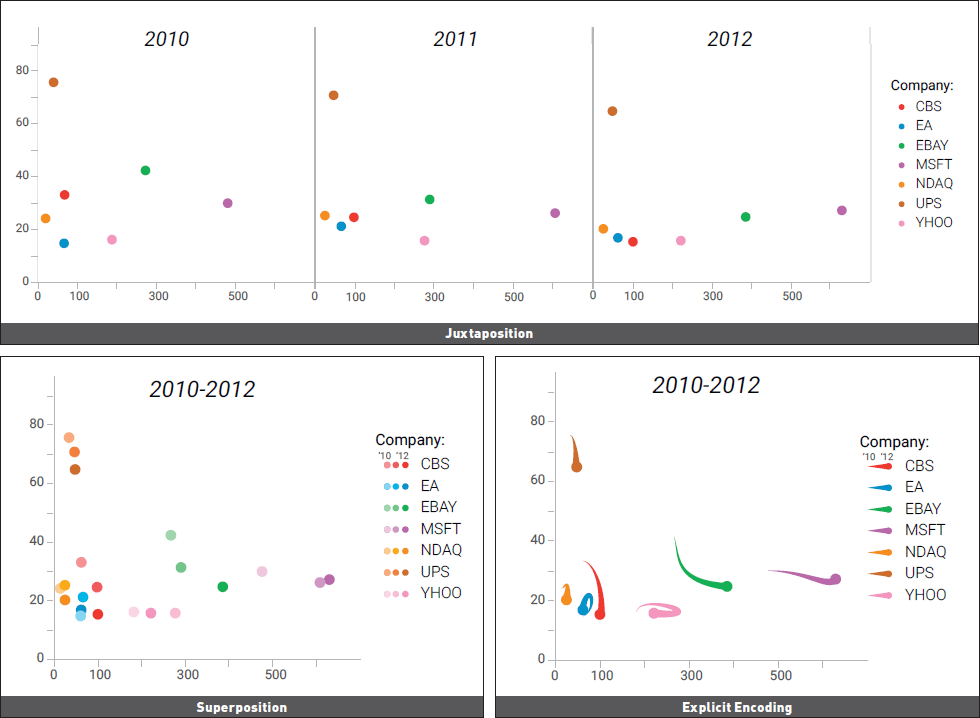
\includegraphics[width=\textwidth]{explicit_encoding}
  \caption{Juxtaposition, Superposition and Explicit Encoding. Image taken from the work of~\cite{Szafir2018}.}
  \label{fig:explicit-endoding-szafir}
\end{figure}

\begin{figure}[H]
  \centering
  \begin{subfigure}[t]{0.75\textwidth}
    \centering
    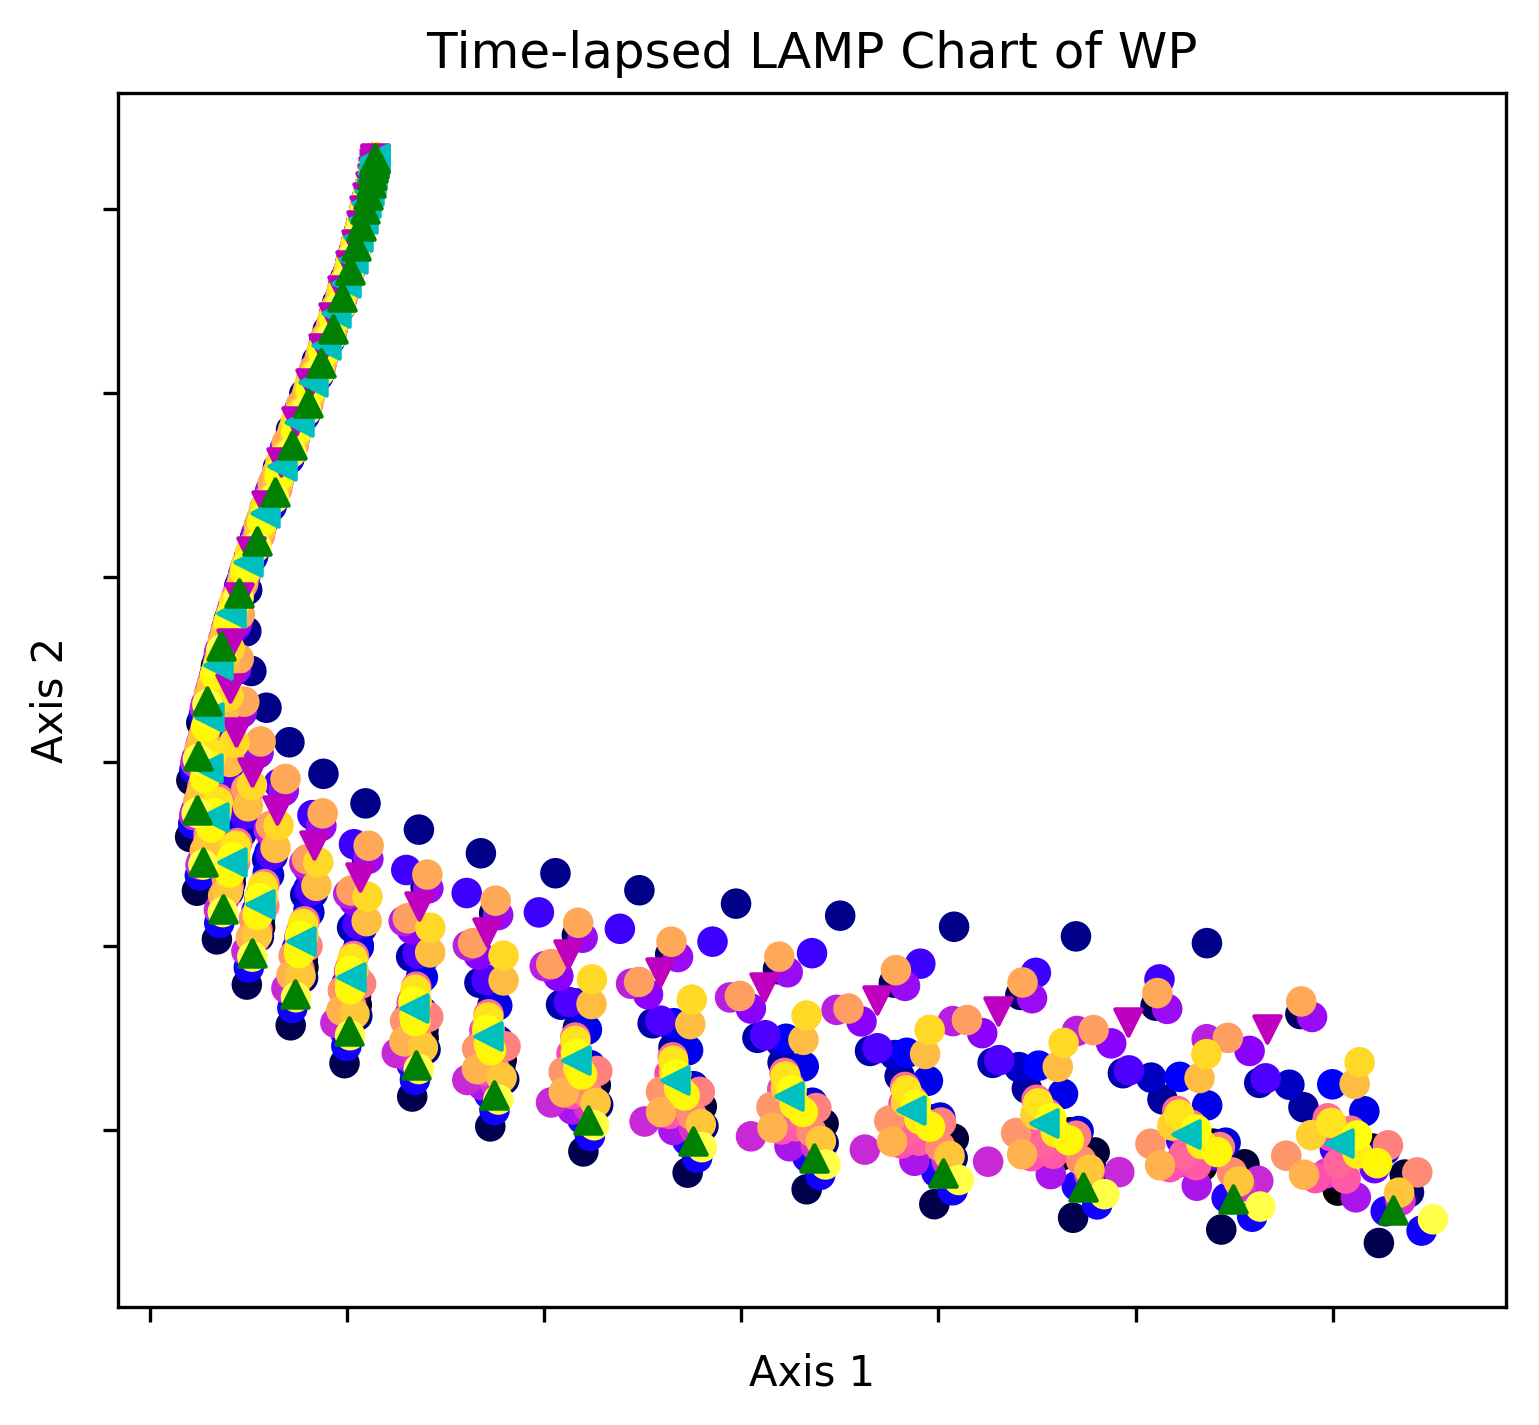
\includegraphics[width=\columnwidth]{WP-tllamp}
    \caption{Superposition of times in the Time-lapsed LAMP chart.}
    \label{fig:superposition-tllamp-inc}
  \end{subfigure}
  ~
  \begin{subfigure}[t]{0.75\textwidth}
    \centering
    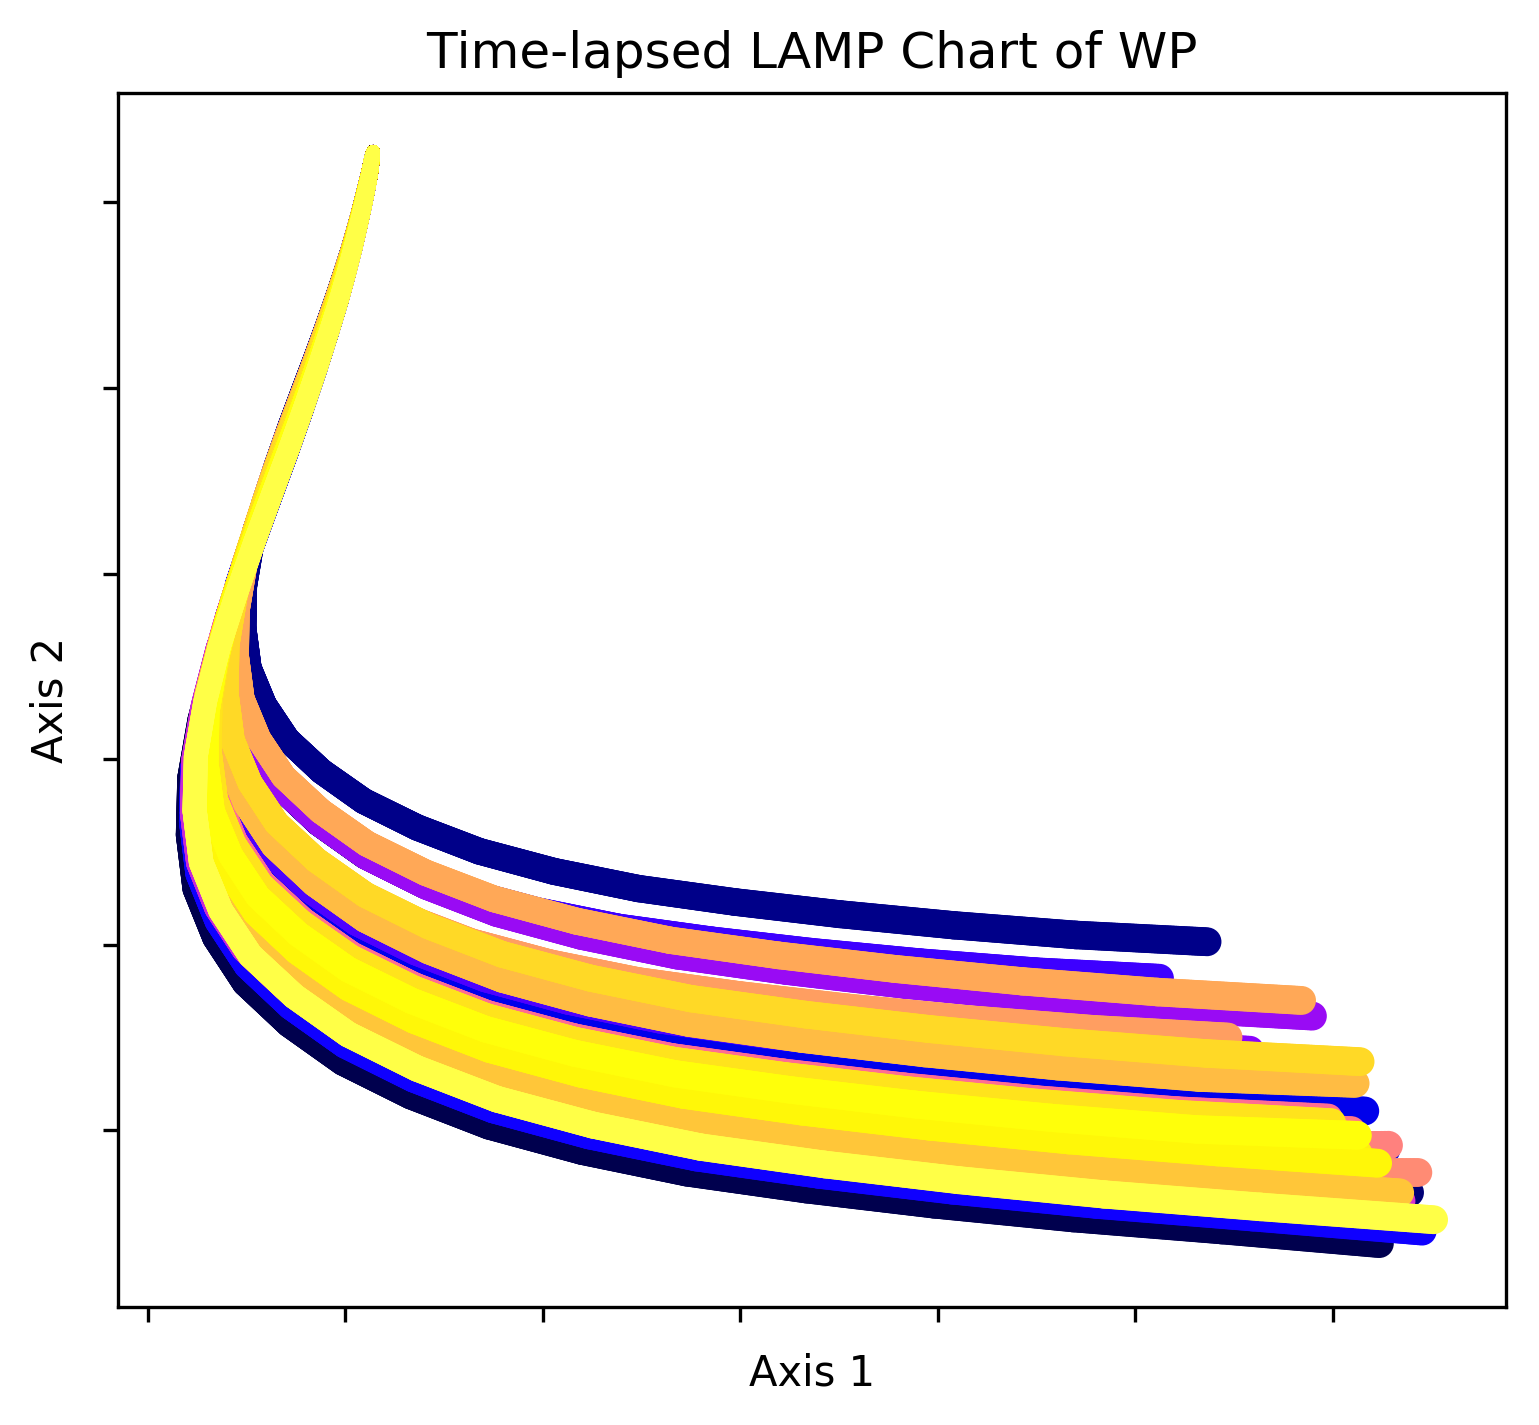
\includegraphics[width=\columnwidth]{WP-tllamp-linear-inc-glyph}
    \caption{Explicit encoding of time in the Time-lapsed LAMP chart. Starting times encoded with smaller glyphs.}
    \label{fig:ee-tllamp-inc}
  \end{subfigure}
  \caption{Comparison between different time encodings on the Time-lapsed LAMP chart of $W_p$. Superposition~(\ref{fig:superposition-tllamp-inc}) and Explicit Encoding~(\ref{fig:ee-tllamp-inc}) from small to large glyphs.}
  \label{fig:explicit-encoding-tllamp-inc}
\end{figure}

%%% Local Variables:
%%% mode: latex
%%% TeX-master: thesis.tex
%%% End:


\arial
\bibliography{../../common/references}

\normalfont
\appendix
\newpage

\chapter{Perfil de usuário para sessão de avaliação do protótipo}
\label{chap:profile-form}

\begin{enumerate}
\item Informações pessoais
  \begin{enumerate}
  \item Nome
    \newline \rule[0pt]{300pt}{1pt}
  \item E-mail
    \newline \rule[0pt]{300pt}{1pt}
  \item Nível de escolaridade
    \newline \rule[0pt]{300pt}{1pt}
  \item Período do curso (apenas para cursos em andamento)
    \newline \rule[0pt]{300pt}{1pt}
  \item Profissão
    \newline \rule[0pt]{300pt}{1pt}
  \end{enumerate}
\item Marque a seguir o seu conhecimento sobre os assuntos
  \begin{enumerate}
  \item Divisão de amostras por percentis: P10, P50, P80 ...
    \newline \circle{10} Desconheço
    \newline \circle{10} Conheço pouco (aprendi esses conceitos em algum momento, mas talvez tenha que aprender novamente se tiver que aplicá-los)
    \newline \circle{10} Tenho conhecimento médio (talvez tenha que rever um ou outro conceito se tiver que aplicá-lo)
    \newline \circle{10} Conheço bem (não aplico com frequência, mas não precisaria rever os conceitos se tivesse que aplicá-los)
    \newline \circle{10} Sou especialista (aplico esses conceitos com frequência)
    \newline 
  \item Análise de tendências e padrões em séries temporais
    \newline \circle{10} Desconheço
    \newline \circle{10} Conheço pouco (aprendi esses conceitos em algum momento, mas talvez tenha que aprender novamente se tiver que aplicá-los)
    \newline \circle{10} Tenho conhecimento médio (talvez tenha que rever um ou outro conceito se tiver que aplicá-lo)
  \end{enumerate}
\end{enumerate}

\end{document}